\documentclass[12pt]{article}

% set indentation
\usepackage{parskip}
%\setlength{\parindent}{16mm}

% for the figures
\usepackage{graphicx}
\usepackage{extsizes}
\usepackage{wrapfig}
% change margins
\usepackage{geometry}
\geometry{left=20mm,right=20mm,top=15mm,bottom=15mm}

% for the reference
\usepackage[sort]{natbib}
\usepackage{url}
\usepackage{placeins}
%\usepackage{authblk}
\usepackage{setspace}
\usepackage{tabularx}
%\doublespacing
% in preamble
%\usepackage{movie15}
% in documenet

\usepackage{authblk}
\usepackage{graphicx}
\usepackage{mathptmx} 
% My packages
\usepackage{parskip}
\usepackage{relsize, threeparttable}
\usepackage{array}
\usepackage{booktabs}
\usepackage{lscape}
\usepackage{tabularx}
\usepackage{makecell}
\usepackage{booktabs}
\usepackage{numprint}
\usepackage{amsmath}
\usepackage{mathtools}
\usepackage{amssymb}
\usepackage{multirow}
\setlength{\parindent}{16mm}
% for the figures
\usepackage{graphicx}
\usepackage{placeins}
% for the reference
\usepackage{natbib}
\usepackage{floatrow}
\usepackage{chngcntr}
\usepackage{url}
\usepackage{dutchcal}
%\usepackage{boondox-calo}
\usepackage{upgreek}
%\date{}
\usepackage{color,soul}
\usepackage{amsmath}

\setlength{\parindent}{0pt}
\definecolor{lightgrey}{rgb}{0.925, 0.925, 0.925}
\sethlcolor{lightgrey}







\title{Unravelling the contribution of financial and longevity risks to changes over time in life annuities}

\author[1]{Jes\'us-Adri\'an \'Alvarez\thanks{alvarez@sdu.dk}}

\author[2]{Andr\'es M. Villegas}

\affil[1]{{\small Interdisciplinary Centre on Population Dynamics, University of Southern Denmark} }

\affil[2]{\small{School of Risk and Actuarial Studies and ARC Centre of Excellence in Population Ageing Research (CEPAR)\\ UNSW Business School, Sydney, Australia}}
%\date{}

\begin{document}
\maketitle

{
\setcounter{tocdepth}{2}
%\tableofcontents
}



\begin{abstract}
	Actuaries and risk managers are interested in developing strategies to ensure that changes in interest rates do not affect the value of a portfolio (commonly known as immunization). Similarly, there is a long-standing tradition among demographers to measure how changes over time in mortality affect summary measures such as life expectancy. In this paper, we bring these two perspectives together. We develop a new decomposition method to quantify the contribution of changes in mortality and interest rates to the change in life annuity prices. We introduce neat and intuitive formulations that allow actuaries and risk managers to easily asses stochastic changes in financial and longevity risks embedded in their life annuities' portfolios. \\
	
	To illustrate our method, we look at the long-term development of life annuity prices using financial and mortality data from the United Kingdom since 1841. We found that there is clear interplay between longevity and financial risk, where the former one is at times masked by high financial risk. 
\end{abstract}
\newpage
\section{Introduction}\label{introduction}


Mortality and interest rates are the driving forces behind fluctuations over time in life annuity prices (factors maybe?). Who contributes the most to such changes, mortality or interest rates? This question depends on many factors such as the onset age of calculation of life annuities, time frame of analysis and, of course, the population to be analysed. However, even by considering all those factors, there is not such a tool to disentangle the sources of stochastic change in life annuity factors. The main reason for this is that fluctuations in mortality and interest rates and their impact in life annuities have been widely studied separately but rarely together.



\subsection*{Demographic perspective on changes in mortality}


The association between changes in mortality and changes in summary measures of longevity such as life expectancy ($e_x$) has hold attention of mathematical demographers and population biologists for many decades \citep{leser1955variations,keyfitz1968introduction,keyfitz1977difference,demetrius1974demographic,mitra1978short,goldman1986new,Vaupel1986,hakkert1987life,fernandez2015entropy}. In particular, \citet{leser1955variations,demetrius1974demographic,keyfitz1977difference} introduced an indicator known as the life table entropy (denoted by \textit{H}), that  “measures changes in life expectancy consequent on a proportional change in the force of mortality, $\mu$” \citep{Keyfitz1985}. The entropy is the elasticity of life expectancy to changes in mortality (the higher the entropy; the higher the sensitivity of ex to death rates), but it is also useful to measure lifespan variation across populations \citep{vaupel2011life,aburto2019threshold,aburto2020dynamics}. Given the dimensionless property of the entropy ($H$ does not depend on the absolute value of $e_x$), this indicator has proved to be adequate in the comparison of age at death distribution across species \citep{baudisch2011pace,wrycza2015quantifying,colchero2016emergence}.


Along the same lines, several demographers have been interested in decomposing changes over time in life expectancy \citep{arriaga1984measuring,pollard1988decomposition,beltran2008integrated,beltran2011unifying}. Key among these contributions is the work done by \citet{Vaupel2003} who develop a neat method in continuous time to separate change life expectancy over time in terms of the general pace of mortality improvement, $\bar{\rho}$, and the entropy, $H$. The advantage of \citet{Vaupel2003} decomposition method relies on the fact that it allows further decomposition of age-specific and cause-specific contributions into the average pace of mortality improvement and entropy.


\subsection*{Longevity and interest rates immunization}



The concept of entropy \citep{leser1955variations,demetrius1974demographic,keyfitz1977difference} was first extended to the case of life annuity ($\bar{a}_x$) by \citet{Haberman2011}. In the context of longevity immunization (strategies to ensure that the value of a portfolio will be little affected in response to changes in death rates), \citet{,wang2010optimal,tsai2011actuarial,Tsai2013a,Li2011} derive discrete formulas for entropy (or what they call mortality durations) and convexities with respect to constant and proportional changes in the force of mortality, $\mu$. Longevity immunization (also called mortality immunization) has been recently extended to different types of life insurance and annuity products \citep{li2012key,Li2012,Wong2015,Luciano2015,levantesi2018natural}. The growing interest on longevity immunization is due to the current scenario that developed countries are facing: low interest rates and continuous mortality improvements. These two factors expose life annuities (and other life contingent products) to higher longevity risk, allowing the capital market of mortality-link securities to grow \citep{blake2019still}.


Financial risk (unexpected changes in interest rates), on the other hand, has been extensively assessed in the context of interest rate immunization \citep{redington1951papers,fisher1971coping,shiu1990redington,santomero1997financial,courtois2007immunization}. This type of immunization is centred on duration (denoted by $D$), which measures the sensitivity of a life annuity (or any other financial product) to changes in the force of interest, $\delta$ \citep{milevsky2013life,charupat2016sluggish}. Modified ($\dfrac{\dfrac{\bar{a}_x}{\delta}}{\bar{a}_x}$) and dollar durations ($\dfrac{\bar{a}_x}{\delta}$) are the most used types of durations in finance. Both assume parallel shifts in the force of interest (WE SHOULD ELABORATE MORE HERE).



\subsection*{Bringing both perspectives together}

Literature on analysis of sensitivity in mortality (mostly developed by mathematical demographers) and literature on sensitivity to interest rates (mostly developed by actuaries and financial managers) have remained largely disconnected\footnote{with exception of \citet{Haberman2011} that made clear the links between both literatures}. Paradoxically, both strands of literature direct efforts at the same objective: better understanding of the inherent sources of risks in life contingent instruments. Recently, \citet{lin2020natural} made strides on this regard by deriving discrete formulas to calculate sensitivity of life annuities (and whole life insurances) to simultaneous changes mortality and interest rates. They introduced a synthetic variable called 'the force of mortality-interest`, which results from the addition of the force of mortality and interest ($\mu^*=\mu+\delta$). While the application of \citet{lin2020natural} is interesting since it combines sensitivity in mortality and interest rates, it is unlikely that $\mu$ and $\delta$ change at the same pace over time.

In this study, we bring together the demographic and actuarial/financial perspectives. We develop a new decomposition method to quantify the contribution of stochastic changes in mortality and interest rates to stochastic changes in life annuity prices. We introduce neat and intuitive formulations that allow actuaries and risk managers to easily asses stochastic changes in financial and longevity risks embedded in their life annuities' portfolios. To illustrate our method, we first look at the long-term development of life annuity prices using financial and mortality data from the United Kingdom since 1841. Next, we forecast trends in mortality and interest rates under various scenarios to gain insights about how both components interplay in future life annuity prices. From the actuarial perspective, our formulations are useful in devising strategies for better risk management (longevity and financial) by levering on well-known results from mathematical demography and immunization.






\section{Preliminaries}\label{preliminaries}

All of the quantities expressed here vary over time $t$. According to standard actuarial notation, we define the following quantities:

\begin{itemize}

\item
\(\mu(x,t)\) is the force of mortality at age \(x\).

\item
$_sp_x(t)=e^{-\int_{0}^{s}\mu(x+y,t)dy}$ is the probability of surviving from age \(x\) to age \(x+s\).


\item
\(\delta(s,t)\) is the force of interest at time $s$. This measure is a general form to express the term-structure of interest rates.

\item 

${v}(s,t)=e^{-\int_{0}^{s}\delta(s,t)dy}$ is the discount factor, where $s$ is the length of the interval from issue of the life annuity to death.

\end{itemize}

The derivative with respect to time $t$ is denoted by adding a point on top of the function of interest. For example, time derivatives for the forces of mortality and interest are expressed as:

\begin{equation} \label{eq:mudot}
\dot{\mu}(x,t)\equiv\frac{\partial\mu(x,t)}{\partial t},
\end{equation}

and 

\begin{equation} \label{eq:mudot}
\dot{\delta}(s,t)\equiv\frac{\partial\delta(s,t)}{\partial t}.
\end{equation}



The rate of mortality improvement (or progress in reducing mortality) is defined as


\begin{equation} \label{eq:rho}
\rho(x,t)=-\frac{\frac{\mu(x,t)}{\partial t}}{\mu(x,t)} = - \frac{\dot{\mu}(x,t)}{\mu(x,t)}.
\end{equation}

Similarly, the relative change in interest rates over time is captured by 


\begin{equation} \label{eq:phi}
\upvarphi(s,t)=-\frac{\frac{\delta(s,t)}{\partial t}}{\delta(s,t)} = -\frac{\dot{\delta}(s,t)}{\delta(s,t)}.
\end{equation}


The actuarial present value of a life annuity at age $x$ evaluated at time $t$ is given by

\begin{equation}\label{eq:Annuity}
\bar{a}_x(t) = \int_0^\infty {}_sp_x(t) {v}(s,t)ds = \int_0^\infty {}_sE_x(t) ds,
\end{equation}

where ${}_sE_x(t)={}_sp_x(t) {v}(s,t)$. 



A life annuity deferred $s$ years starting to be paid at age $x+s$ is expressed as


\begin{equation}\label{eq:DefAnnuity}
{}_s|\bar{a}_x(t) = {}_sE_x(t) \bar{a}_{x+s}(t)
\end{equation}


\section{Dynamics of a life annuity}


We are interested on measuring changes in $\bar{a}_x(t)$ with respect to the time variable $t$. To achieve this aim, we first need to describe how $\bar{a}_x(t)$ reacts to changes in the forces of mortality and interest. We denote the \textit{entropy of a life annuity}\footnote{\cite{Tsai2011,Tsai2013a,Lin2020} denoted this measure as \textit{mortality duration}. We reserve the term duration to denote changes in $\bar{a}_x(t)$ with respect to interest rates.} as the measure that captures changes in $\bar{a}_x(t)$ with respect to $\mu(x,t)$. Formally, it is defined as 

\begin{equation}\label{eq:EntropyGeneral}
{H}_{x}(t) = \frac{ \frac{\partial \bar{a}_x(t) }{\partial \mu(x,t)}}{\bar{a}_x(t)}.
\end{equation}

The measure that captures the sensitivity of $\bar{a}_x(t)$ to changes in interest rates is commonly known as \textit{duration} and it is the foundation of interest rates' immunization. For a life annuity, it is defined as the relative derivative of the annuity factor with respect to changes in the force of interest \citep{Milevsky2012}:


\begin{equation}\label{eq:DurationGeneral}
{D}_{x}(t) = \frac{ \frac{\partial \bar{a}_x(t) }{\partial \delta(s,t)}}{\bar{a}_x(t)}.
\end{equation}

Greater values for ${H}_{x}(t)$ and ${D}_{x}(t)$ indicate that $\bar{a}_x(t)$ is highly sensitive to changes in $\mu(x,t)$ and $\delta(s,t)$ respectively. The entropy and the duration of a life annuity can be measured either by assuming constant or proportional changes in $\mu(x,t)$ and $\delta(s,t)$. In the following section we develop formulations for both cases. 



\subsection{Changes in $\bar{a}_x(t)$ with respect to $\mu(x,t)$}

The entropy of a life annuity is denoted by ${H}^{c}_{x}(t)$ when changes in $\mu(x,t)$ are held constant at all ages and by ${H}^{p}_{x}(t)$ when  changes are performed proportional. Based on the results developed by \citet{Tsai2013a} and \citet{Lin2020}, when $\mu(x,t)$ is changed constantly to $\mu(x,t)+\gamma$ such that $\gamma$ is a small number (see proof in the Appendix), the entropy of $\bar{a}_x(t)$ becomes

\begin{equation}\label{eq:EntropyC}
{H}^{c}_{x}(t) = -\frac{\int_{0}^\infty s {}_sp_x(t) {v}(s,t) ds}{\bar{a}_x(t)}=\frac{{h}^{c}_{x}(t)}{\bar{a}_x(t)},
\end{equation}

where ${h}^{c}_{x}(t)=-\int_{0}^\infty s {}_sp_x(t) {v}(s,t) ds$. The term ${h}^{c}_{x}(t)$ is expressed in absolute (monetary) terms, whereas the entropy ${H}^{c}_{x}(t)$ is dimensionless because it does not depend on the absolute value of $\bar{a}_x(t)$.


In two separate articles, \citet{Haberman2011} and \citet{Tsai2013a} show that when changes in $\mu(x,t)$ are assumed to be proportional to a small number $\gamma$ such that $\mu(x,t)(1+\gamma)$, the entropy of $\bar{a}_x(t)$ becomes

\begin{equation} \label{eq:EntropyP}
{H}^{p}_{x}(t) = -\frac{ \int_{0}^{\infty}{}_sp_x(t)\ln[{}_sp_x(t)] {v}(s,t) ds}{\int_0^\infty {}_sp_x(t) {v}(s,t) ds}.
\end{equation}


Alternatively, we show (see proof in Section \ref{sec:EntropyAlt} of the Appendix) that Equation \ref{eq:EntropyP} can be expressed as

\begin{equation} \label{eq:EntropyP2}
\begin{split}
{H}^{p}_{x}(t) &=  \frac{\int_0^\infty \mu(x+s,t)   {}_s|\bar{a}_x(t) ds}{\bar{a}_x(t)} =  \frac{{h}^{p}_{x}(t)}{\bar{a}_x(t)}, 
\end{split}
\end{equation}

where ${h}^{p}_{x}(t)=\int_0^\infty \mu(x+s,t)   {}_s|\bar{a}_x(t) ds$. Analogous to the case where changes are assumed to be constant, quantities ${h}^{p}_{x}(t)$ and ${H}^{p}_{x}(t)$ are expressed in absolute and relative terms respectively. The formulations shown in this section are closely related to the ones developed in the mortality immunization literature \citep{Tsai2013a,Lin2020}. We extended them to the continuous case.

 
 

\subsection{Changes in $\bar{a}_x(t)$ with respect to $\delta(s,t)$}

 Similar to the entropy, changes in $\bar{a}_x(t)$ with respect to $\delta(s,t)$ can be assumed to be either constant or proportional. Duration assuming constant changes in $\delta(s,t)$ is denoted by ${D}^{c}_{x}(t)$, whereas ${D}^{p}_{x}(t)$ refers to the duration assuming proportional changes. For the former case we have that:



\begin{equation}\label{eq:DurationC}
\begin{split}
{D}^{c}_x(t)&= -\frac{\int_0^\infty s {}_sp_x(t) {v}(s,t)ds}{\bar{a}_x(t)} \\
&= \frac{{d}^{c}_x(t)}{\bar{a}_x(t)},
\end{split}
\end{equation}

where ${d}^{c}_x(t)=-\int_0^\infty s {}_sp_x(t) {v}(s,t)ds$. Thus, assuming constant changes in $\delta(s,t)$ results into common types of duration known in finance as \textit{dollar duration}, ${d}^{c}_x(t)$, and \textit{modified duration}, ${D}^{c}_x(t)$ (see \citet{Milevsky2012} and \citet{Tsai2013a} for further details). It is worth noting that Equations \ref{eq:EntropyC} and \ref{eq:DurationC} are identical such that ${d}^{c}_x(t)={h}^{c}_{x}(t)$. This means that constant (parallel) changes in the force of mortality have essentially the same effect as parallel changes in the force of interest.


Assuming proportional changes in $\delta(s,t)$ (see proof in Section \ref{sec:DurProp} of the Appendix) results in: 


\begin{equation}\label{eq:DurationP}
\begin{split}
{D}^{p}_{x}(t) &= -\frac{\int_0^\infty {}_sp_x(t) v(s,t) \ln(v(s,t))ds}{\bar{a}_x(t)}. \\
\end{split}
\end{equation}


Note that when assuming constant force of mortality such that $v(s,t)=e^{-\delta(t)s}$, we have that ${D}^{p}_{x}(t)=\delta(t){D}^{c}_{x}(t)$,


\begin{equation}\label{eq:DurationCP}
\begin{split}
{D}^{p}_{x}(t) &= -\frac{\int_0^\infty {}_sp_x(t) v(s,t) \ln(v(s,t))ds}  {\bar{a}_x(t)} \\
&=- \delta(t)\frac{\int_0^\infty s{}_sp_x(t) e^{-\delta(t)s}  ds}{\bar{a}_x(t)} \\
& = \delta(t){D}^{c}_{x}(t).
\end{split}
\end{equation}

Equation \ref{eq:DurationP} can also be re-expressed as:

\begin{equation}\label{eq:DurationP2}
\begin{split}
{D}^{p}_{x}(t) &= \frac{\int_0^\infty \delta(s,t) {}_s|\bar{a}_x(t)ds} {\bar{a}_x(t)} \\
                 &= \frac{{d}^{p}_{x}(t)}{\bar{a}_x(t)}.
\end{split}
\end{equation}


where ${d}^{p}_{x}(t)=\int_0^\infty \delta(s,t) {}_s|\bar{a}_x(t) ds$. 




\section{Time derivative of $\bar{a}_x(t)$} \label{sec:timderiv}

We compute the derivative of $\bar{a}_x(t)$ with respect to the time variable $t$, $\dot{\bar{a}} _x(t)=\frac{\partial \bar{a}_x(t)}{\partial t}$, such that

\begin{equation}\label{eq:TimeDeriv}
\begin{split}
\dot{\bar{a}} _x(t) &= \int_0^\infty {}_s\dot{p}_x(t) v(s,t)ds +\int_0^\infty {}_sp_x(t) \dot{v}(s,t)ds.\\
\end{split}
\end{equation}


To develop a closed-form solution for Equation \ref{eq:TimeDeriv} we consider the general case where $_sp_x(t)=e^{-\int_{0}^{s}\mu(x+y,t)dy}$ and ${v}(s,t)=e^{-\int_{0}^{s}\delta(s,t)dy}$. We analyse separately each of the two terms in the right side of Equation \ref{eq:TimeDeriv}. Let us first focus on the first term:


\begin{equation}\label{eq:TimeDerivP1}
\begin{split}
\int_0^\infty {}_s\dot{p}_x(t) v(s,t) &= \int_0^\infty   v(s,t) e^{-\int_0^{s}\dot{\mu}(x+y,t)dy}ds\\
&= -\int_0^\infty   v(s,t) {}_sp_x(t)\int_0^{s}\dot{\mu}(x+y,t)dyds\\
&= -\int_0^\infty  \dot{\mu}(x+s,t) \int_s^{\infty} v(y,t) {}_yp_x(t) dyds\\
&= - \int_0^\infty \dot{\mu}(x+s,t)   {}_sE_x(t) \bar{a} _{x+s}(t) ds\\
&= \int_0^\infty \rho(x+s,t) \mu(x+s,t)   {}_s|\bar{a}_x(t) ds\\
\end{split}
\end{equation}


The second part equals:

\begin{equation}\label{eq:TimeDerivP2}
\begin{split}
\int_0^\infty {}_sp_x(t) \dot{v}(s,t)ds &= \int_0^\infty {}_sp_x(t)  e^{-\int_0^{s}\dot{\delta}(y,t)dy}ds\\
&= -\int_0^\infty {}_sp_x(t) v(s,t) \int_0^{s}\dot{\delta}(y,t)dy ds\\
&= -\int_0^\infty  \dot{\delta}(s,t)\int_s^{\infty} {}_yp_x(t) v(y,t) dy ds\\
&= \int_0^\infty  \upvarphi(s,t) \delta(s,t)  {}_s|\bar{a}_x(t) ds\\
\end{split}
\end{equation}


Thus, $\dot{\bar{a}} _x(t)$ can be expressed as


\begin{equation}\label{eq:TimeDerivP3}
\begin{split}
\dot{\bar{a}}_{x}(t) &=  \int_0^\infty \rho(s,t) \mu(s,t){}_s|\bar{a}_x(t) ds +\int_0^\infty  \upvarphi(s,t) \delta(s,t)  {}_s|\bar{a}_x(t) ds\\
&= \int_0^\infty \rho(s,t) {}_sM_x(t)  ds +\int_0^\infty  \upvarphi(s,t) {}_sW_x(t)  ds,
\end{split}
\end{equation}


where ${}_sM_x(t)= \mu(s,t){}_s|\bar{a}_x(t)$ and ${}_sW_x(t)=\delta(s,t)  {}_s|\bar{a}_x(t)$. We can express Equation \ref{eq:TimeDerivP3} in terms of the duration and entropy


\begin{equation}\label{eq:TimeDerivP}
\begin{split}
 \acute{\bar{a}}_x(t) = \frac{\dot{\bar{a}}_x(t)}{\bar{a}_x(t)}  = 
 \underbrace{\bar{\rho}(t){H}^{p}_x(t)}_\text{longevity component}
 +\underbrace{\bar{\upvarphi}(t){D}^{p}_x(t),}_\text{financial component}
\end{split}
\end{equation}

where $\bar{\rho}(t)= \frac{\int_0^\infty \rho(s,t) {}_sM_x(t)  ds}{\int_0^\infty  {}_sM_x(t)ds}$ and 
$\bar{\upvarphi}(t)= \frac{\int_0^\infty \upvarphi(s,t) {}_sW_x(t)  ds}{\int_0^\infty {}_sW_x(t) ds}$ are the average paces of change in mortality and interest rates respectively. Functions $\bar{\rho}(t)$ and $\bar{\upvarphi}(t)$ capture the stochastic change in the forces of mortality and interest whereas ${H}^{p}_x(t)$ and ${D}^{p}_x(t)$ capture the sensitivity due to changes in $\mu$ and $\delta$. In other words, Equation \ref{eq:TimeDerivP} entails that changes over time in $\bar{a}_x(t)$ are driven by $\bar{\rho}(t)$ and $\bar{\upvarphi}(t)$, which are modulated by ${H}^{p}_x(t)$ and ${D}^{p}_x(t)$ respectively. Equation \ref{eq:TimeDerivP} is an extension of the decomposition formula to changes over time in life expectancy developed by \citet{Vaupel2003}. Here we extended it to life annuities.



\subsection{Assuming constant force of interest}


It is common to use a single interest rate (without using the term-structure of interest rates, $\delta(s,t)$) for the calculation of life annuity factors. Thus, we re-express the decomposition formula for $\acute{\bar{a}}_x(t)$ by assuming $v(s,t)=e^{-\delta(t)s}$. This assumption affects only the second part of Equation \ref{eq:TimeDeriv}: 




\begin{equation}\label{eq:TimeDerivC1}
\begin{split}
\int_0^\infty {}_s{p}_x(t) \dot{v}(s,t)ds &=\int_0^\infty {}_s{p}_x(t) \frac{\partial \left[ e^{-\delta(t)s} \right]}{\partial t}ds \\
&=-\dot{\delta}(t)\int_0^\infty s  {}_s{p}_x(t) e^{-\delta(t)s} ds \\
&=  \dot{\delta}(t)  d^{c}_x(t).
\end{split}
\end{equation}

Substituting Equations \ref{eq:TimeDerivP1} and \ref{eq:TimeDerivC1} in Equation \ref{eq:TimeDeriv} results into: 


\begin{equation}\label{eq:TimeDerivC2}
\begin{split}
\acute{\bar{a}}_x(t) =  \bar{\rho}(t){H}^{p}_x(t)+\dot{\delta}(t)  D^{c}_x(t).
\end{split}
\end{equation}



Given that ${D}^{p}_{x}(t)=\delta(t){D}^{c}_{x}(t)$ (see Equation \ref{eq:DurationCP}), it is straight-froward to show that in the case of a single interest rate, Equations \ref{eq:TimeDerivP}  and \ref{eq:TimeDerivC2} are equivalent. Thus, it suffices to use the entropy (${H}^{p}_x(t)$) and the modified duration ($D^{c}_x(t)$) together with $\bar{\rho}(t)$ and $\dot{\delta}(t)$ to determine the contribution of financial and longevity risks to changes over time in life annuities.





\subsection{Recap of formulations}




\textbf{[Here I am planning to add a table with all the formulas]}

\section{Historical contribution of mortality and interest to changes in life annuities}



In this section we illustrate the decomposition method developed in Section \ref{sec:timderiv} by examining the long-term development of life annuities in the UK. We use two centuries of data from 1841 to 2018. Age-specific death rates come from the \citep{HMD2020}. Long-term interest rates are represented by the yield on 2.5\% Consols up to 1977, then by the yield on FTSE Actuaries Government Securities Irredeemable stocks up to 2014 and thereafter by the yield on FTSE Actuaries Government Securities 45 years stock (INCLUDE REFERENCE). We calculated life annuity factors at ages 65, 70 and 75 to understand how the longevity and financial components react to different onset ages.

\begin{figure}[!ht]
	\centering
	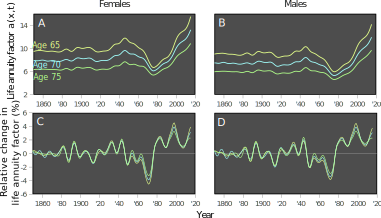
\includegraphics[width=1\textwidth]{Fig/Fig1}
	\caption{\textit{Trends over time in life annuity factors and relative change in $\bar{a}_x(t)$ calculated at ages 65, 70 and 75. Both sexes, 1841-2018.}}
	\label{fig:Fig1}
\end{figure}


How has the value of life annuities changed over time? Panels A and B of Figure \ref{fig:Fig1} depict values for $\bar{a}_x(t)$ from 1841 to 2018 calculated at ages 65, 70 and 75 for females and males respectively. We observe that during the second half of the 19th century and up to the decade of 1940s, $\bar{a}_x(t)$ remained at similar levels with small fluctuations. Thereafter, $\bar{a}_x(t)$ exhibited a sharp decline up to the decade of 1980s followed by an increasing pattern that has remained until recent years.
  
Sex-specific trends appear to be very similar between sexes with the absolute level of $\bar{a}_x(t)$ for females being slightly higher than the one depicted for males. Similar trends over time also replicate at any onset age of calculation analysed here (e.g. age 65, 70 and 75). However, a closer look reveal that $\bar{a}_x(t)$ changes more abruptly at younger ages (age 65) than at older ages (age 75). This pattern is clear when analysing the time derivative of $\bar{a}_x(t)$ portrayed by $\acute{\bar{a}}_x(t)$  (see Panels C and D of Figure 1). In the following sections we analyse the sources of the time trend in  $\acute{\bar{a}}_x(t)$ by making use of the decomposition method developed in Section \ref{sec:timderiv}.

\subsection{Contribution of financial and longevity risks to changes in $\bar{a}_x(t)$}

According to the decomposition formula developed (Equation \ref{eq:TimeDerivC2}), changes over time in $\bar{a}_x(t)$ can be explained in terms of longevity and financial components. Each component depends on the stochastic fluctuations of $\mu(x,t)$ and $\delta(s,t)$ (captured by $\bar{\rho}(t)$ and $\dot{\delta}(t)$ respectively) which are modulated by the sensitivity of $\bar{a}_x(t)$ to changes in the forces of mortality and interest (entropy, ${H}^{p}_x(t)$ and modified duration, ${D}^{c}_x(t)$). We first describe sex-specific trends in $\dot{\delta}(t)$ and $\bar{\rho}(t)$ (see Figure \ref{fig:Fig2}). 



\begin{figure}[!ht]
	\centering
	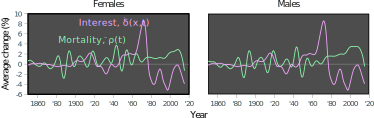
\includegraphics[width=1\textwidth]{Fig/Fig2}
	\caption{\textit{Average change in mortality ($\bar{\rho}(t)$) calculated for all ages above age 65 and rate of change in interest rates ($\dot{\delta}(t)$). Note that $\dot{\delta}(t)$ is expressed in basis points to ease readability. Both sexes, 1841-2018.}}
	\label{fig:Fig2}
\end{figure}


Time trends for $\bar{\rho}(t)$ are very much alike at ages 65, 70 and 75. Hence, we only focus on $\bar{\rho}(t)$ at age 65 to illustrate the general change in mortality. Values for rho at ages 70 and 75 can be found in the Appendix (ADD THIS). During most of the observation period, $\bar{\rho}(t)$ fluctuated between 0\% and 2\%. As of 1980s, $\bar{\rho}(t)$ remained steady indicating an average mortality improvement above age 65 of 2\% and 3\% for the decade of 2000s. In recent years, $\bar{\rho}(t)$ trended downwards, which coincides with the mortality deterioration currently prevailing in the United Kingdom (REF). 

Regarding changes over time in the force of interest, we observe that $\dot{\delta}(t)$ has also remained at similar levels for most of the observation period with some fluctuations between 1930 and 1950. Since the 1960s, $\dot{\delta}(t)$ went up rapidly reaching the highest increase (of around 8\% in the decade of 1970s). Thereafter, $\dot{\delta}(t)$ declined faster and moved towards negative values entailing a decline in interest rates, which is still ongoing until recent time. As mentioned above, $\bar{\rho}(t)$ and $\dot{\delta}(t)$ are responsible for the time trend we observe in $\bar{a}_x(t)$, which is modulated by the entropy, ${H}^{p}_x(t)$, and modifed duration, ${D}^{c}_x(t)$.



\begin{figure}[!ht]
	\centering
	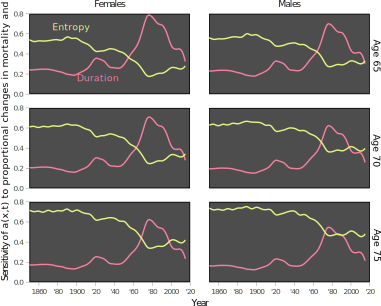
\includegraphics[width=1\textwidth]{Fig/Fig3}
	\caption{\textit{Entropy and modified duration assuming proportional changes calculated at ages 65, 70 and 75. Both sexes, 1841-2018.}}
	\label{fig:Fig3}
\end{figure}



From Figure \ref{fig:Fig3}, we observe that ${H}^{p}_x(t)$ and ${D}^{c}_x(t)$ have fluctuated over time. The entropy went down for most of the observation period and up to the 1980s where it started to rise. Modified duration, on the other hand, remained somewhat constant over time with a small peak in the 1920s. However, as of the 1950s ${D}^{c}_x(t)$ trended upwards reaching its maximum in the 1980s (of about 0.8) and then begin to drop. It is worth noting that there are some specific points in time where ${H}^{p}_x(t)$ and ${D}^{c}_x(t)$ are equal. This means that $\bar{a}_x(t)$ is equally sensitive to changes in mortality and interest rates.

From Figure \ref{fig:Fig3}, the interplay between ${H}^{p}_x(t)$ and ${D}^{c}_x(t)$ is clear. We observe two regularities. First, ${H}^{p}_x(t)$ is lower for females than for males whereas ${D}^{c}_x(t)$ is higher for females than for males. This means that, in general, $\bar{a}_x(t)$ for females is less sensitive to $\mu$ and more sensitive to $\delta$ than for males. Second, $\bar{a}_x(t)$ becomes more sensitive to $\mu$ (higher ${H}^{p}_x(t)$) and less sensitive to $\delta$ (lower ${D}^{c}_x(t)$) when calculating $\bar{a}_x(t)$ at older ages. This finding is key to understand how the contributions of longevity and financial risks are moderated differently across ages.


\begin{figure}[!ht]
	\centering
	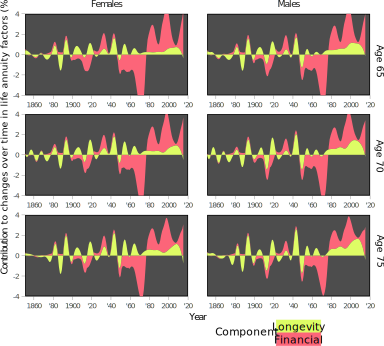
\includegraphics[width=1\textwidth]{Fig/Fig4}
	\caption{\textit{Decomposition of changes over time in life annuity factors calculated at ages 65, 70 and 75. Both sexes, 1841-2018.}}
	\label{fig:Fig4}
\end{figure}



Figure \ref{fig:Fig4} depicts the contribution of financial ($\dot{\delta}(t){D}^{c}_x(t)$) and longevity ($\bar{\rho}(t){H}^{p}_x(t)$) components (SHOULD WE CALL THEM RISKS??) to changes in $\bar{a}_x(t)$ calculated at ages 65, 70 and 75. Positive/negative values contribute to increase/decrease in $\bar{a}_x(t)$. Both, longevity and financial component have played an important role on long-term development of $\bar{a}_x(t)$. 

From Figure \ref{fig:Fig4} we can distinguish among 5 important periods where life annuity prices fluctuated (\ref{fig:Fig1}) in response to specific changes in mortality and interest rates (\ref{fig:Fig2}). From 1841 to 1945 we observe stable annuity prices with year on year fluctuations. Decreasing annuity prices driven by increase in interest rates that masked mortality improvements are observed from 1945 to 1970. Next, annuity prices trended upwards from 1945 to 1970 driven by both interest rates increases and mortality improvements. From 2000 to 2015 we observe a peak contribution of longevity with most contributions to changes driven by mortality rates. From 2015 onwards, increase in prices driven by falling interest rates have masked the reduction in prices resulting from the deceleration of mortality improvement. It is worth noting that longevity contributions to changes in $\bar{a}_x(t)$ are more pronounced in males than in females throughout the whole period of observation.

From Figure \ref{fig:Fig4} we observe When looking at $\bar{a}_x(t)$ calculated at different ages, we observe that the longevity component takes more relevance at older ages. For example, we observe that in recent years the longevity component is responsible for a greater contribution of changes in $\bar{a}_{75}(t)$ than for changes in $\bar{a}_{65}(t)$. This pattern is magnified for males. All in all, Figure \ref{fig:Fig4} provides evidence of the contribution of financial and longevity components to changes in the long-term development of life annuity factors.









\FloatBarrier
\section{Projection of the decomposition of changes in annuities}









\newpage

\bibliographystyle{apalike}
%\bibliography{/Users/Jesus/Documents/Papers/BibTex/Proposal}
%\bibliography{C:/Users/jmartinez/OneDrive - Syddansk Universitet/Papers/BibTeX/Proposal.bib}

\bibliography{library}

\newpage

\appendix
\section{Appendix}



\subsection{Entropy with constant changes in $\mu(x+s,t)$}\label{sec:EntropyConst}

To measure constant changes we make $\mu(s,t)+\gamma$, then

\begin{equation}\label{eq:EntropyConst1}
\begin{split}
\bar{a}_{x}(t) &= \int_0^\infty{v}(s,t) e^{-\int_{0}^{s} [\mu(x+y,t)+\gamma]dy}ds \\
&= \int_0^\infty {v}(s,t)e^{-\int_{0}^{s} \mu(x+y,t)dy} e^{-\gamma s}ds \\
&= \int_0^\infty {v}(s,t){}_sp_x(t) e^{-\gamma s}ds \\
\end{split}
\end{equation}

We expand $e^{-\gamma s}$ to $1-\gamma s+\frac{\gamma^2}{2} s^{2} +...$, so that


\begin{equation}\label{eq:EntropyConst2}
\begin{split}
\bar{a}_{x}(t) &= \int_0^\infty {}_sp_x(t) {v}(s,t)[1-\gamma s+\frac{\gamma^2}{2} s^{2} +...]ds
\end{split}
\end{equation}

We take the derivative $\bar{a}_{x}(t)$ with respect to $\gamma$ and evaluate $\gamma=0$


\begin{equation}\label{eq:EntropyConst3}
\begin{split}
{H}^{c}_x(t)&=\frac{1}{\bar{a}_x(t)}\frac{\partial \bar{a}_x(t)}{\partial \gamma} \bigg\rvert_{\gamma=0}\\
&= -\frac{\int_0^\infty s {}_sp_x(t) {v}(s,t)ds}{\bar{a}_x(t)} \\
&= \frac{{h}^{c}_x(t)}{\bar{a}_x(t)},
\end{split}
\end{equation}

where ${h}^{c}_x(t)=-\int_0^\infty s {}_sp_x(t) {v}(s,t)ds$



\subsection{Alternative expression for ${H}^{p}_{x}(t)$}\label{sec:EntropyAlt}

\begin{equation} \label{eq:EntropyAnnuityA1}
\begin{split}
{H}^{p}_{x}(t) &= -\frac{ \int_{0}^{\infty}{}_sp_x(t)\ln[{}_sp_x(t)] e^{-\int_{0}^{s}\delta(y,t)dy} ds}{\int_0^\infty {}_sp_x(t) e^{-\int_{0}^{s}\delta(y,t)dy} ds}\\
&= \frac{\int_0^\infty {}_sp_x(t) {v}(s,t) \int_0^s \mu(x+y,t) dy\,ds}{\bar{a}_x(t)}\\
&= \frac{\int_0^\infty  \mu(x+s,t) \int_s^\infty {}_yp_x(t) {v}(y,t)  dy\,ds}{\bar{a}_x(t)}\\
&= \frac{\int_0^\infty  \mu(x+s,t)  {}_sp_x(t) {v}(s,t) \int_s^\infty \frac{ {}_yp_x(t) {v}(y,t)}{ {}_sp_x(t) {v}(s,t)}  dy\,ds}{\bar{a}_x(t)}\\
&=  \frac{\int_0^\infty \mu(x+s,t)   {}_sp_x(t) {v}(s,t) \bar{a}_{x+s}(t) ds}{\bar{a}_x(t)} \\
&=  \frac{\int_0^\infty \mu(x+s,t)  {}_s|\bar{a}_x(t) ds}{\bar{a}_x(t)} \\
&=  \frac{{h}^{p}_{x}(t)}{\bar{a}_x(t)}, \\
\end{split}
\end{equation}

where ${h}^{p}_{x}(t)=\int_0^\infty \mu(x+s,t)   {}_s|\bar{a}_x(t) ds$.



\subsection{Duration with constant changes in $\delta(s,t)$}\label{sec:DurConst}

To measure constant changes we make $\delta(s,t)+\gamma$, then

\begin{equation}\label{eq:DurationConst1}
\begin{split}
\bar{a}_{x}(t) &= \int_0^\infty {}_sp_x(t) e^{- \int_{0}^{s} [\delta(y,t)+\gamma]dy}ds \\
&= \int_0^\infty {}_sp_x(t) e^{- \int_{0}^{s}\delta(y,t)dy}e^{-\gamma s}ds \\
&= \int_0^\infty {}_sp_x(t) {v}(s,t)e^{-\gamma s}ds
\end{split}
\end{equation}

We expand $e^{-\gamma s}$ to $1-\gamma s+\frac{\gamma^2}{2} s^{2} +...$, so that


\begin{equation}\label{eq:DurationConst1}
\begin{split}
\bar{a}_{x}(t) &= \int_0^\infty {}_sp_x(t) {v}(s,t)[1-\gamma s+\frac{\gamma^2}{2} s^{2} +...]ds
\end{split}
\end{equation}

We take the derivative $\bar{a}_{x}(t)$ with respect to $\gamma$ and evaluate $\gamma=0$


\begin{equation}\label{eq:DurationConst2}
\begin{split}
{D}^{c}_x(t)&=-\frac{1}{\bar{a}_x(t)}\frac{\partial \bar{a}_x(t)}{\partial \gamma} \bigg\rvert_{\gamma=0}\\
              &= \frac{\int_0^\infty s {}_sp_x(t) {v}(s,t)ds}{\bar{a}_x(t)} \\
              &= \frac{{d}^{c}_x(t)}{\bar{a}_x(t)},
\end{split}
\end{equation}

where ${d}^{c}_x(t)=\int_0^\infty s {}_sp_x(t) {v}(s,t)ds$



\subsection{Duration with proportional changes in $\delta(s,t)$} \label{sec:DurProp}

To calculate duration with proportional changes in $\delta(s,t)$, we assume that $\gamma$ is a small number such that $\delta(s,t)(1+\gamma)$ and  ${v}(s,t)=e^{-\int_0^{s}  \delta(y,t)(1+\gamma)dy}$.


\begin{equation}\label{eq:DurationProp1}
\begin{split}
\bar{a} _x(t) &= \int_0^\infty {}_sp_x(t) e^{-\int_0^{s}\delta(y,t)(1+\gamma)dy}ds \\
&= \int_0^\infty {}_sp_x(t) e^{-\int_0^{s}\delta(y,t)dy}e^{-\int_0^{s}\delta(y,t)\gamma dy}ds \\
&= \int_0^\infty {}_sp_x(t) v(s,t)v(s,t)^{\gamma}ds \\
\end{split}
\end{equation}


We expand $v(s,t)^{\gamma}$ to $1+\ln(v(s,t)) \gamma+{\ln(v(s,t))}^2 \frac{\gamma^2}{2}+...$, so that


\begin{equation}\label{eq:DurationProp2}
\begin{split}
\bar{a}_x(t) &= \int_0^\infty {}_sp_x(t) s(y,t)[1+\ln(v(s,t)) \gamma+{\ln(v(s,t))}^2 \frac{\gamma^2}{2}+...]ds\\
\end{split}
\end{equation}


To calculate the duration ${D}^{p}_{x}(t)$ we take the derivate of the expression above with respect to $\gamma$ and make $\gamma=0$

\begin{equation}\label{eq:DurationProp3}
\begin{split}
{D}^{p}_{x}(t)&=-\frac{1}{\bar{a}_x(t)}\frac{\partial \bar{a}_x(t)}{\partial \gamma} \bigg\rvert_{\gamma=0} \\
&= -\frac{\int_0^\infty {}_sp_x(t) v(s,t) \ln(v(s,t))ds}{\bar{a}_x(t)} \\
\end{split}
\end{equation}


Equation \ref{eq:DurationProp3} can be re-expressed as 


\begin{equation}\label{eq:DurationProp4}
\begin{split}
{D}^{p}_{x}(t) &= -\frac{\int_0^\infty {}_sp_x(t) v(s,t) \ln(v(s,t))ds}{\bar{a}_x(t)}\\
&= \frac{\int_0^\infty {}_sp_x(t) v(s,t) \int_0^{s} \delta(y,t)dy ds }{\bar{a}_x(t)}\\
&= \frac{\int_0^\infty \delta(s,t)  \int_{s}^{\infty} {}_{y}p_x(t) v(y,t)dy ds }{\bar{a}_x(t)}\\
&= \frac{\int_0^\infty \delta(s,t) {}_sp_x(t) v(s,t) \bar{a}_{x+s}(t)  ds }{\bar{a}_x(t)}\\
&= \frac{\int_0^\infty \delta(s,t) {}_s|\bar{a}_x(t) ds}{\bar{a}_x(t)} \\
&= \frac{{d}^{p}_{x}(t)}{\bar{a}_x(t)}.
\end{split}
\end{equation}



where ${d}^{p}_{x}(t)=\int_0^\infty \delta(s,t) {}_s|\bar{a}_x(t) ds$.


\end{document}
